\section{Live GPS receiver-to-position pipeline}
\label{sec:live}
\textbf{LIVE-GPS-L1-R1} supplies the actual GPS equations and transport inputs
missing from the prepared-observation kernel. The implemented chain is
\begin{equation}
\text{RTCM bytes}\longrightarrow(P_i,e_i,t_r)
\longrightarrow(x_{s,i}^{rx},\delta t_{s,i},I_i,T_i)
\longrightarrow(x_r,y_r,z_r,b_r).
\end{equation}
The raw code $P_i$ and satellite ephemeris $e_i$ come from a real remote receiver;
the physical corrections are calculated locally. The orbit and atmospheric model
is Python; the position/clock solution is the existing FP64 native CPU/CUDA
kernel, reached through a persistent process. This closes the reception-to-position
chain without assuming an upstream program has already solved the geometry.

\begin{panel}
\textbf{Meaning of the live demonstration}\par
The user has no local GNSS hardware. The Internet supplies observations from
the LIENSS reference receiver in the public Centipede network. Every computed
coordinate in this experiment locates that remote receiver. Its transmitted
antenna reference point (ARP) is held out of the estimator and used only for
subsequent comparison. No host-computer location is inferred from it.
\end{panel}

\subsection{What crosses the network boundary}
The bounded client performs a read-only NTRIP/HTTP GET, or reads a TCP byte stream.
It supports HTTP chunk framing, optional ICY headers, timeouts and bounded
reconnection. Centipede permits one NTRIP client per public IP; the recorded
CPU and GPU sessions run sequentially. The public service is documented at
\href{https://docs.centipede.fr/docs/centipede/3_connect_caster.html}{Centipede: connecting to the caster}.
The exact source URL, bytes, UTC reception records, connection boundaries and
SHA-256 fingerprints accompany each capture. No local coordinate/GGA is sent.

RTCM3 uses preamble \code{D3}, a ten-bit payload length and CRC24Q with
polynomial \code{0x1864CFB}. CRC is transport-error detection, not authentication.
The implemented receiver extracts GPS LNAV message 1019; station metadata
1005/1006; legacy GPS code 1004; and GPS MSM4/5/6/7 (1074--1077). Other
constellation MSM messages are consumed so their terminal flags correctly close
the shared observation epoch. Their measurements do not enter the GPS-only solve.

An epoch is keyed by station ID and full GPST time. The multiple-message flag
keeps fragments together until a terminal fragment arrives. CRC loss, reconnect,
changed epoch before termination and end-of-input produce explicit incomplete
records. RTCM has no fragment count or sequence-start flag: a newly connected
client cannot prove that it saw the first fragment. This limitation is retained
in the event metadata; missing ranges are not reconstructed from station geometry.

The one selected signal per satellite is C1C (L1 C/A), mapped to channel
$i=\mathrm{PRN}-1$. MSM7's finer positive pseudorange takes precedence over
legacy 1004 for the same signal. A valid legacy value may fill an unavailable
MSM value. All original signal fields are retained; zero, absent or invalid code
does not become a solver row. Carrier phase is decoded/preserved where present
but no ambiguity state is estimated by this profile.

\subsection{Time, provenance and reproducible execution}
Times are unwrapped GPS seconds from 1980-01-06. RTCM week ambiguity is resolved
against the recorded reception date, with an explicit GPS-minus-UTC offset of
18 seconds for these sessions. This value is stated by
\href{https://maia.usno.navy.mil/information/eo-values}{USNO Earth-orientation values};
it is a configurable input, not an automatically maintained leap-second service.
RINEX epochs already tagged GPST receive no additional UTC offset.

No RTCM 1019 message contains the Klobuchar coefficients. The demonstrated
sessions use only the GPSA/GPSB header of the same-day BKG broadcast file
\path{BRDC00WRD_R_20262570000_01D_MN.rnx}:
\begin{align}
\alpha&=(1.2107\!\times\!10^{-8},\ 1.4901\!\times\!10^{-8},\
 -5.9605\!\times\!10^{-8},\ -1.1921\!\times\!10^{-7}),\\
\beta&=(96256,\ 81920,\ -196610,\ -393220).
\end{align}
Its orbital records are \emph{not} loaded during RTCM operation. Every usable
satellite orbit/clock arrives in message 1019 from the stream itself. Download
URLs, UTC acquisition time and hashes are in the source-data manifests. With no
ionosphere header, the model explicitly labels its 5 ns baseline approximation.

Run the included Windows CPU worker from the release directory:
\begin{lstlisting}
python tools/live_satnav.py
  --binary bin/cpu/satnav_stream.exe
  --url ntrip://caster.centipede.fr:2101/LIENSS
  --iono-nav source/live_data/
    BRDC00WRD_R_20262570000_01D_MN.rnx
  --seconds 180 --out results/my_live_run
\end{lstlisting}
The display wraps one command for readability; join it onto one line and keep
the navigation-file path continuous. Select the CUDA binary and add
\code{--backend cuda} for the GPU path. Use a new output directory for each run.
The dated ionosphere file reproduces this experiment; future-day operation
should supply a current header or explicitly select the documented fallback.

The same final received bytes can be replayed with an explicit full-time reference:
\begin{lstlisting}
python tools/live_satnav.py
  --binary bin/cpu/satnav_stream.exe
  --rtcm source/live_data/
    centipede_lienss_20260914/capture.rtcm3
  --reference-gpst 1473457283
  --iono-nav source/live_data/
    BRDC00WRD_R_20262570000_01D_MN.rnx
  --out results/my_recorded_run
\end{lstlisting}
RINEX input uses \code{--rinex-obs} and \code{--nav}; it is explicitly recorded
as file replay. The input contract, all optional arguments, live-to-CGK bridge
and independent oracle commands are supplied in \path{docs/LIVE_INPUT.md},
\path{docs/LIVE_HANDOFF.md} and the source-data README.

\clearpage
\subsection{LIVE-R1 time contract and broadcast orbit}
\label{sec:live-orbit}

A raw observation is $(t_r^{\rm tag},P_i,\mathrm{PRN}_i,\sigma_{0i})$.
Time is full, unwrapped GPS seconds from 1980-01-06; $P_i$ is the original
GPS L1 C/A pseudorange in metres. Receiver time tags and code share one clock
convention. GPS-labelled RINEX calendar fields receive no UTC conversion.
The final physical reception-time estimate is
\begin{equation}
 \widehat t_r=t_r^{\rm tag}-\widehat b_r/c,
 \qquad c=299\,792\,458\ \mathrm{m\,s^{-1}}.
 \label{eq:live-reception-time}
\end{equation}
Here $b_r$ is the estimated receiver clock bias in metres. The raw tag remains
in the trace. RTCM week rollover is resolved against an explicit reception-date
reference; age tests use full time, never a modulo-week age.

Each GPS ephemeris provides $\sqrt A,e,i_0,\Omega_0,\omega,M_0,\Delta n,
\dot i,\dot\Omega$, six harmonic coefficients, $t_{oe},t_{oc}$, three clock
coefficients, $T_{GD}$, health and issue identifiers. The selected record has
matching PRN, healthy status and $\mathrm{IODC}\bmod256=\mathrm{IODE}$.
Both clock and orbit age are bounded by $7200$ s; a shorter declared half-fit
interval further limits orbit age. A nearer unhealthy issue is not replaced
by an older healthy issue.

For signal emission time $t_s$, define
\begin{align}
 A&=(\sqrt A)^2,&t_k&=t_s-t_{oe},\\
 n&=\sqrt{\mu/A^3}+\Delta n,&M&=M_0+n t_k,
 \qquad \mu=3.986005\times10^{14}\ \mathrm{m^3\,s^{-2}}.
\end{align}
Newton's method solves $E-e\sin E=M$:
\begin{equation}
 E_{j+1}=E_j-\frac{E_j-e\sin E_j-M}{1-e\cos E_j}.
\end{equation}
The implementation reduces $M$ modulo $2\pi$, starts at $E_0=M$, and requires
an increment below $10^{-14}$ rad within 30 iterations. For $0\leq e<1$,
\begin{align}
 \nu&=\operatorname{atan2}\!\left(\sqrt{1-e^2}\sin E,\cos E-e\right),
 &\phi&=\nu+\omega,\\
 u&=\phi+C_{us}\sin2\phi+C_{uc}\cos2\phi,\\
 r&=A(1-e\cos E)+C_{rs}\sin2\phi+C_{rc}\cos2\phi,\\
 i&=i_0+\dot i\,t_k+C_{is}\sin2\phi+C_{ic}\cos2\phi,\\
 \Omega&=\Omega_0+(\dot\Omega-\omega_e)t_k
                  -\omega_e(t_{oe}\bmod604800),\\
 \omega_e&=7.2921151467\times10^{-5}\ \mathrm{rad\,s^{-1}}.
\end{align}
All angles are radians. Radius harmonics are metres; the other harmonics are
angular corrections. These definitions implement the GPS LNAV user algorithm
in \href{https://www.gps.gov/sites/default/files/2025-07/IS-GPS-200N.pdf}{IS-GPS-200N,
section 20.3.3.4.3}; they are new GPS-specific additions to this kernel package.

\clearpage
\subsection{Satellite clock, emission time and reception axes}
\label{sec:live-clock}

Let $x'=r\cos u$ and $y'=r\sin u$. The satellite position in the Earth-fixed
axes at emission is
\begin{equation}
 \widetilde{\boldsymbol x}_s=
 \begin{pmatrix}
 x'\cos\Omega-y'\cos i\sin\Omega\\
 x'\sin\Omega+y'\cos i\cos\Omega\\
 y'\sin i
 \end{pmatrix}.
\end{equation}
With $\Delta t_c=t_s-t_{oc}$, the broadcast clock polynomial, eccentric-orbit
relativity correction, and L1 code clock are
\begin{align}
 \delta t_{\rm poly}&=a_{f0}+a_{f1}\Delta t_c+a_{f2}\Delta t_c^2,\\
 \delta t_{\rm rel}&=F e\sqrt A\sin E,
 &F&=-4.442807633\times10^{-10}\ \mathrm{s\,m^{-1/2}},\\
 \delta t_{s,L1}&=\delta t_{\rm poly}+\delta t_{\rm rel}-T_{GD}.
 \label{eq:live-l1-clock}
\end{align}
The trace stores all three contributions separately. The $-T_{GD}$ sign is
specific to this L1 profile. An external differential C1--P1 bias is not
invented. Alternate code types are rejected until their signal-bias model is
explicit. See \href{https://www.gps.gov/sites/default/files/2025-07/IS-GPS-200N.pdf}{IS-GPS-200N,
sections 20.3.3.3.3.1--20.3.3.3.3.2}.

The measured code connects the receiver and satellite clock tags:
\begin{equation}
 t_s^{\rm tag}=t_r^{\rm tag}-P/c,
 \qquad
 t_s^{(j+1)}=t_s^{\rm tag}-\delta t_{s,L1}(t_s^{(j)}).
 \label{eq:live-transmit-time}
\end{equation}
The adapter uses three clock iterations starting at $t_s^{\rm tag}$. The
receiver clock cancels in $t_r^{\rm tag}-P/c$, because it occurs in both raw
quantities. Subtracting the receiver clock again here would double-correct the
emission time. This construction follows ESA's
\href{https://gssc.esa.int/navipedia/index.php/Emission_Time_Computation}{pseudorange-based
emission-time algorithm}.

Earth rotation over the travel time is applied once, before the native solve:
\begin{align}
 R_3(a)&=\begin{pmatrix}\cos a&\sin a&0\\-\sin a&\cos a&0\\0&0&1\end{pmatrix},\\
 \boldsymbol x_s^{rx}&=R_3(\omega_e\tau)\widetilde{\boldsymbol x}_s,
 &\tau&=\|\boldsymbol x_s^{rx}-\boldsymbol x_r\|/c.
 \label{eq:live-earth-rotation}
\end{align}
Four range iterations, initially $\tau_0=P/c$, determine the reception-frame
satellite position for the current receiver estimate. The native model never
rotates it a second time. The rotation sign and frame convention follow
\href{https://gssc.esa.int/navipedia/index.php/Satellite_Coordinates_Computation}{ESA's
reception-frame coordinate construction}.

The first GSI epoch supplies an independent component check: all eight
emission positions match the native RTKLIB trace within $0.000578$ m and its
clock values within $0.000438$ ns. The RTKLIB trace rounds coordinates to
millimetres and clocks to $0.001$ ns, and excludes $T_{GD}$ from its reported
satellite clock. The comparison therefore adds $T_{GD}$ back to
Equation~\eqref{eq:live-l1-clock} for that check only.

\clearpage
\subsection{Complete Klobuchar L1 ionosphere}
\label{sec:live-ionosphere}

WGS84 ECEF-to-geodetic conversion supplies receiver latitude $\varphi_r$,
longitude $\lambda_r$ and ellipsoidal height $h$. Rotating the line of sight
into local ENU gives azimuth $A_z$ clockwise from north and elevation
$\mathcal E$. A default $10^\circ$ elevation mask is applied after the receiver
geometry has been initialized.

Klobuchar latitude, longitude and elevation arguments are in semicircles:
$\varphi_u=\varphi_r/\pi$, $\lambda_u=\lambda_r/\pi$ and
$\epsilon=\mathcal E/\pi$. Azimuth remains in radians. The complete pierce-point
and geomagnetic construction is
\begin{align}
 \psi&=\frac{0.0137}{\epsilon+0.11}-0.022,\\
 \varphi_I&=\min\!\left(0.416,
       \max\!\left(-0.416,\varphi_u+\psi\cos A_z\right)\right),\\
 \lambda_I&=\lambda_u+\frac{\psi\sin A_z}{\cos(\pi\varphi_I)},\\
 \varphi_m&=\varphi_I+0.064\cos\!\left(\pi(\lambda_I-1.617)\right),\\
 t_{\rm local}&=(43200\lambda_I+t_r^{\rm tag})\bmod86400.
\end{align}
With the four broadcast alpha and four beta coefficients,
\begin{align}
 A_I&=\max\!\left(0,\sum_{j=0}^{3}\alpha_j\varphi_m^j\right),\\
 P_I&=\max\!\left(72000,\sum_{j=0}^{3}\beta_j\varphi_m^j\right),\\
 X&=\frac{2\pi(t_{\rm local}-50400)}{P_I},\\
 F_I&=1+16(0.53-\epsilon)^3.
\end{align}
Amplitude $A_I$ is seconds and period $P_I$ is seconds. The slant L1 delay,
converted to metres, is
\begin{equation}
 I=cF_I
 \begin{cases}
 5\times10^{-9}+A_I\left(1-X^2/2+X^4/24\right),&|X|<1.57,\\
 5\times10^{-9},&\text{otherwise}.
 \end{cases}
 \label{eq:live-klobuchar}
\end{equation}
Every trigonometric operation on a semicircle value explicitly multiplies by
$\pi$. The limits on pierce latitude, amplitude and period are part of the
published model. See
\href{https://gssc.esa.int/navipedia/index.php/Klobuchar_Ionospheric_Model}{ESA's
Klobuchar equations}, and GPS LNAV ionosphere parameters in
\href{https://www.gps.gov/sites/default/files/2025-07/IS-GPS-200N.pdf}{IS-GPS-200N,
section 20.3.3.5.2.5}.

When broadcast coefficients are unavailable, the adapter explicitly selects
$\alpha_j=\beta_j=0$ and records
\code{klobuchar\_zero\_coefficients\_5ns\_baseline}. This still produces
$cF_I\,5\times10^{-9}$ metres of delay; it is not zero ionosphere. For the
internet capture, an independently downloaded BKG broadcast navigation header
provides the coefficients, with its source hash retained. Receiver ephemerides
can still come from the actual RTCM 1019 stream.

\clearpage
\subsection{Troposphere, observation variance and native solve}
\label{sec:live-observation-equation}

LIVE-R1 uses a specified standard atmosphere with relative humidity $H=0.7$.
For $-100\leq h\leq10000$ m and $\mathcal E>0$, define
\begin{align}
 h_0&=\max(h,0),\\
 p&=1013.25(1-2.2557\times10^{-5}h_0)^{5.2568}\quad[\mathrm{hPa}],\\
 T&=288.16-0.0065h_0\quad[\mathrm K],\\
 e_w&=6.108H\exp\!\left(\frac{17.15T-4684}{T-38.45}\right)
       \quad[\mathrm{hPa}].
\end{align}
The hydrostatic and wet Saastamoinen delays are
\begin{align}
 T_h&=\frac{0.0022768p}
 {(1-0.00266\cos2\varphi_r-0.00028h_0/1000)\sin\mathcal E},\\
 T_w&=\frac{0.002277(1255/T+0.05)e_w}{\sin\mathcal E},
 &T_d&=T_h+T_w.
 \label{eq:live-saastamoinen}
\end{align}
Negative terrestrial heights use sea-level weather and carry a specific status.
Outside the height domain, atmosphere is omitted with an explicit diagnostic;
no calibrated weather is inferred. These constants and equations match the
independent \href{https://github.com/tomojitakasu/RTKLIB/blob/71db0ffa/src/rtkcmn.c}{RTKLIB
\code{tropmodel} source}.

The default nominal code uncertainty is $\sigma_{0i}=3$ m. The executed native
profile weights observations by
\begin{equation}
 \sigma_i=\frac{\sigma_{0i}}{\max(\sin\mathcal E_i,0.1)},
 \qquad W_{ii}=\sigma_i^{-2}.
 \label{eq:live-weight}
\end{equation}
CN0 is retained when supplied, without an invented CN0-to-variance calibration.
These are nominal independent variances, not measured position errors or
protection levels.

The full measurement equation and its single additive correction are
\begin{align}
 P_i&=\|\boldsymbol x_r-\boldsymbol x_{s,i}^{rx}\|+b_r
       -c\delta t_{s,i,L1}+I_i+T_{d,i}+\epsilon_i,\\
 a_i&=c\delta t_{s,i,L1}-I_i-T_{d,i},
 &P_{i,\mathrm{corr}}&=P_i+a_i.
 \label{eq:live-corrected-code}
\end{align}
The native CPU/CUDA solver estimates
$\boldsymbol s=(x_r,y_r,z_r,b_r)^\mathsf T$ by weighted least squares. For
$\rho_i=\|\boldsymbol x_r-\boldsymbol x_{s,i}^{rx}\|$,
\begin{equation}
 r_i=P_{i,\mathrm{corr}}-\rho_i-b_r,
 \qquad
 H_i=\begin{pmatrix}
 (\boldsymbol x_r-\boldsymbol x_{s,i}^{rx})^\mathsf T/\rho_i&1
 \end{pmatrix}.
\end{equation}
An online Givens QR solve of the whitened system gives $\Delta\boldsymbol s$;
$\boldsymbol s\leftarrow\boldsymbol s+\Delta\boldsymbol s$. Rank, iteration,
finite-value and residual-fit results remain explicit. Literal ASA/NA selection
is unchanged, including whole-word absorption on a selected boundary hit.

\clearpage
\subsection{Persistent receiver execution and correction feedback}
\label{sec:live-outer-loop}

The persistent native worker receives complete epochs. The preparation layer
and native solve form the outer state-feedback map
\begin{align}
 \mathcal O_n^{(k)}&=\operatorname{Prepare}
       (P_n,t_n^{\rm tag},\mathcal E_n,\boldsymbol s_n^{(k)}),\\
 \boldsymbol s_n^{(k+1)}&=\operatorname{NativeSolve}
       (\mathcal O_n^{(k)},\boldsymbol s_n^{(k)}),
 \label{eq:live-outer-feedback}
\end{align}
where $\mathcal E_n$ denotes the available ephemeris set. Preparation recomputes
reception-frame geometry, elevation selection, ionosphere, troposphere and
weights from the new position. The default outer limit is eight passes.
A valid position requires initialized terrestrial geometry, a converged native
solve, and
\begin{equation}
 \max\!\left(
 \|\boldsymbol x_n^{(k+1)}-\boldsymbol x_n^{(k)}\|,
 |b_n^{(k+1)}-b_n^{(k)}|
 \right)<10^{-3}\ \mathrm m.
\end{equation}

At the first receiver epoch, the complete state is zero. Geometry initialization
uses all available healthy GPS codes with orbit and clock corrections; the
trace explicitly marks atmosphere and elevation as uninitialized. After the
first coarse Earth position is solved, the next pass activates the physical
models. Reference-station coordinates are never read as seeds. Subsequent
epochs start from this worker's preceding valid solution:
\begin{equation}
 \boldsymbol s_{n+1}^{(0)}=\widehat{\boldsymbol s}_n.
\end{equation}
A failed epoch does not overwrite that state. A detected receiver/station change
resets the seed. Duplicate or out-of-order epochs do not produce a new fix.
This is per-epoch code positioning with a warm start; it does not silently add
a motion prior or carrier-phase ambiguities.

The geometric mechanics profile remains a downstream consumer of position
results. Its JK state is not injected into satellite orbit/clock corrections
or used as a fictitious GNSS observation. The live feedback in
Equation~\eqref{eq:live-outer-feedback} closes the formerly missing receiver
preparation loop around the existing position kernel.

\begin{panel}
\textbf{Separate observable evidence.}
The journal stores raw measurements, every preparation pass, every native
solution and final availability. Correction components retain signs and units.
A recorded-file replay, a local timed replay, and a current internet receiver
stream are distinct source modes. A remote reference receiver's position is
its antenna position; it does not measure the position of the user's computer.
\end{panel}

The GSI 120-epoch run starts at ECEF zero, converges on all epochs, and agrees
with independent NumPy solves of all 263 converged passes within
$1.17\times10^{-8}$ m per state component. The executed weighting differs from
RTKLIB's broadcast-variance weighting: their final positions differ by a mean
$0.529$ m and a maximum $1.589$ m. A controlled NumPy re-solve with the same
physical corrections and RTKLIB weights reduces those differences to a mean
$0.000174$ m and a maximum $0.000346$ m. This experiment isolates the weighting
choice; it is recorded separately from the executed native profile. The full
report is \path{results/real_0759_cpu/independent_comparison.json}.


\subsection{Persistent execution and exact records}
\code{satnav\_stream} starts once and accepts successive complete requests. Each
request contains the epoch ID/time, four-component seed, unchanged ASA/NA/boundary
words and up to 32 observation rows. Replies contain status, fit classification,
ECEF/clock, formal variance, residuals, iteration count and kernel timing. Both
CPU and CUDA dispatch the same SATNAV equations. A rejected request produces an
error record; a Python response timeout closes the worker so a late response
cannot be assigned to the next epoch.

Each completed decoded epoch triggers correction preparation and native solves
while the socket session is still open. There is no whole-file staging step in
the live path. Warm starts carry only the last complete position/clock estimate;
they do not introduce velocity filtering or modify raw ranges. Native failure,
missing ephemeris and exhausted outer correction iterations publish a null
position with an explicit status. Diagnostics still retain the partial iterate.
Fit classification remains separate from numerical convergence.

\begin{center}
\begin{tabularx}{\textwidth}{@{}P{.35\textwidth}Y@{}}\toprule
\textbf{Artifact} & \textbf{Recorded content}\\\midrule
\code{capture.rtcm3} + sidecars & Raw received body, SHA-256, host times and connection boundaries.\\
\code{events.jsonl} & Decoded original fields, orbital issues, station metadata and incomplete/error records.\\
\code{trace.jsonl} & Raw epoch; every preparation and native pass; final position/clock/time and validity.\\
\code{prepared/} & Exact final-pass CSV geometry/corrections for independent Householder and native batch replay.\\
\code{summary.json} & Source identity, counts, worker binary identity, timing scope and capture outcome.\\\bottomrule
\end{tabularx}
\end{center}

Only one synchronous callback operates on received bytes. If decoding, disk I/O
or positioning becomes slower than delivery, TCP backpressure accumulates upstream.
The local demonstration measures a 1 Hz station and is bounded in duration/bytes;
it establishes neither continuous service availability nor a hard real-time bound.
Socket timeouts, CRC/epoch-loss tests and recorded continuity expose the tested
failure semantics. Clock-tag freshness is reported separately from local compute
time: this host's UTC clock was about two seconds behind the incoming GPST tags,
so a negative tag-to-host interval is not interpreted as negative network latency.

\clearpage
\subsection{Current live execution and independent validation}
\label{sec:live-validation}
Both final sessions ran on 14 September 2026 UTC (the local Netherlands date
crossed into 15 September during the work). Each captured 180 complete one-second
epochs using one public caster connection. CPU and CUDA ran sequential sessions:
CPU: 21:55:20--21:58:20 UTC; CUDA: 21:58:54--22:01:54 UTC. The source is \code{caster.centipede.fr:2101/LIENSS}.
\begin{center}
\begin{tabularx}{\textwidth}{@{}P{.61\textwidth}YY@{}}\toprule
\textbf{Measured quantity} & \textbf{CPU} & \textbf{CUDA}\\\midrule
Complete received epochs & 180 & 180\\
Published native positions & 172 & 175\\
Initial unavailable epochs (ephemeris warmup) & 8 & 5\\
Initial ECEF/clock seed & Zero & Zero\\
Mean 3D separation from advertised ARP (m) & 1.644 & 1.854\\
Maximum ARP separation (m) & 2.232 & 2.267\\
Mean 3D difference from RTKLIB (m) & 0.649 & 0.622\\
Maximum RTKLIB difference (m) & 0.969 & 0.931\\
Median complete-input-to-position (ms) & 2.205 & 5.947\\
Maximum complete-input-to-position (ms) & 11.611 & 14.346\\
All positions emitted during socket capture & Yes & Yes\\\bottomrule
\end{tabularx}
\end{center}
The native outputs and their timestamps were checked against the exact raw-frame
hashes and receive-chunk sidecars. The latency above runs from the host receiving
the final required input fragment to publication of a valid position. It includes
local decoding and solving; it is not a calibrated radio/network transit time.
It excludes unavailable warmup epochs. CUDA's first unavailable live epoch took
2.59 seconds inside processing, including initial device work. A separate
persistent-worker regression measured about 1.05 seconds for its first request.
CPU is faster for this small 1 Hz workload; these results establish CUDA correctness,
not a speedup. The CUDA device was the RTX 5070 Ti Laptop, compute capability 12.0,
built with CUDA 12.8 and driver 591.59.

The comparison coordinate is the stream's advertised antenna reference point:
\begin{equation}
 (4426043.0455,\ -89429.1998,\ 4576296.6447)\ \mathrm m.
\end{equation}
It was neither a supplied initial estimate nor an observation. It is not an
independently surveyed truth coordinate in this experiment. Consequently the table
reports separation from advertised ARP, not certified absolute accuracy. RTKLIB
also performs single-point code positioning here; its output quality code is 5,
not an RTK fixed-ambiguity solution.

\clearpage
\subsection{Measured position series and independent checks}
\begin{center}
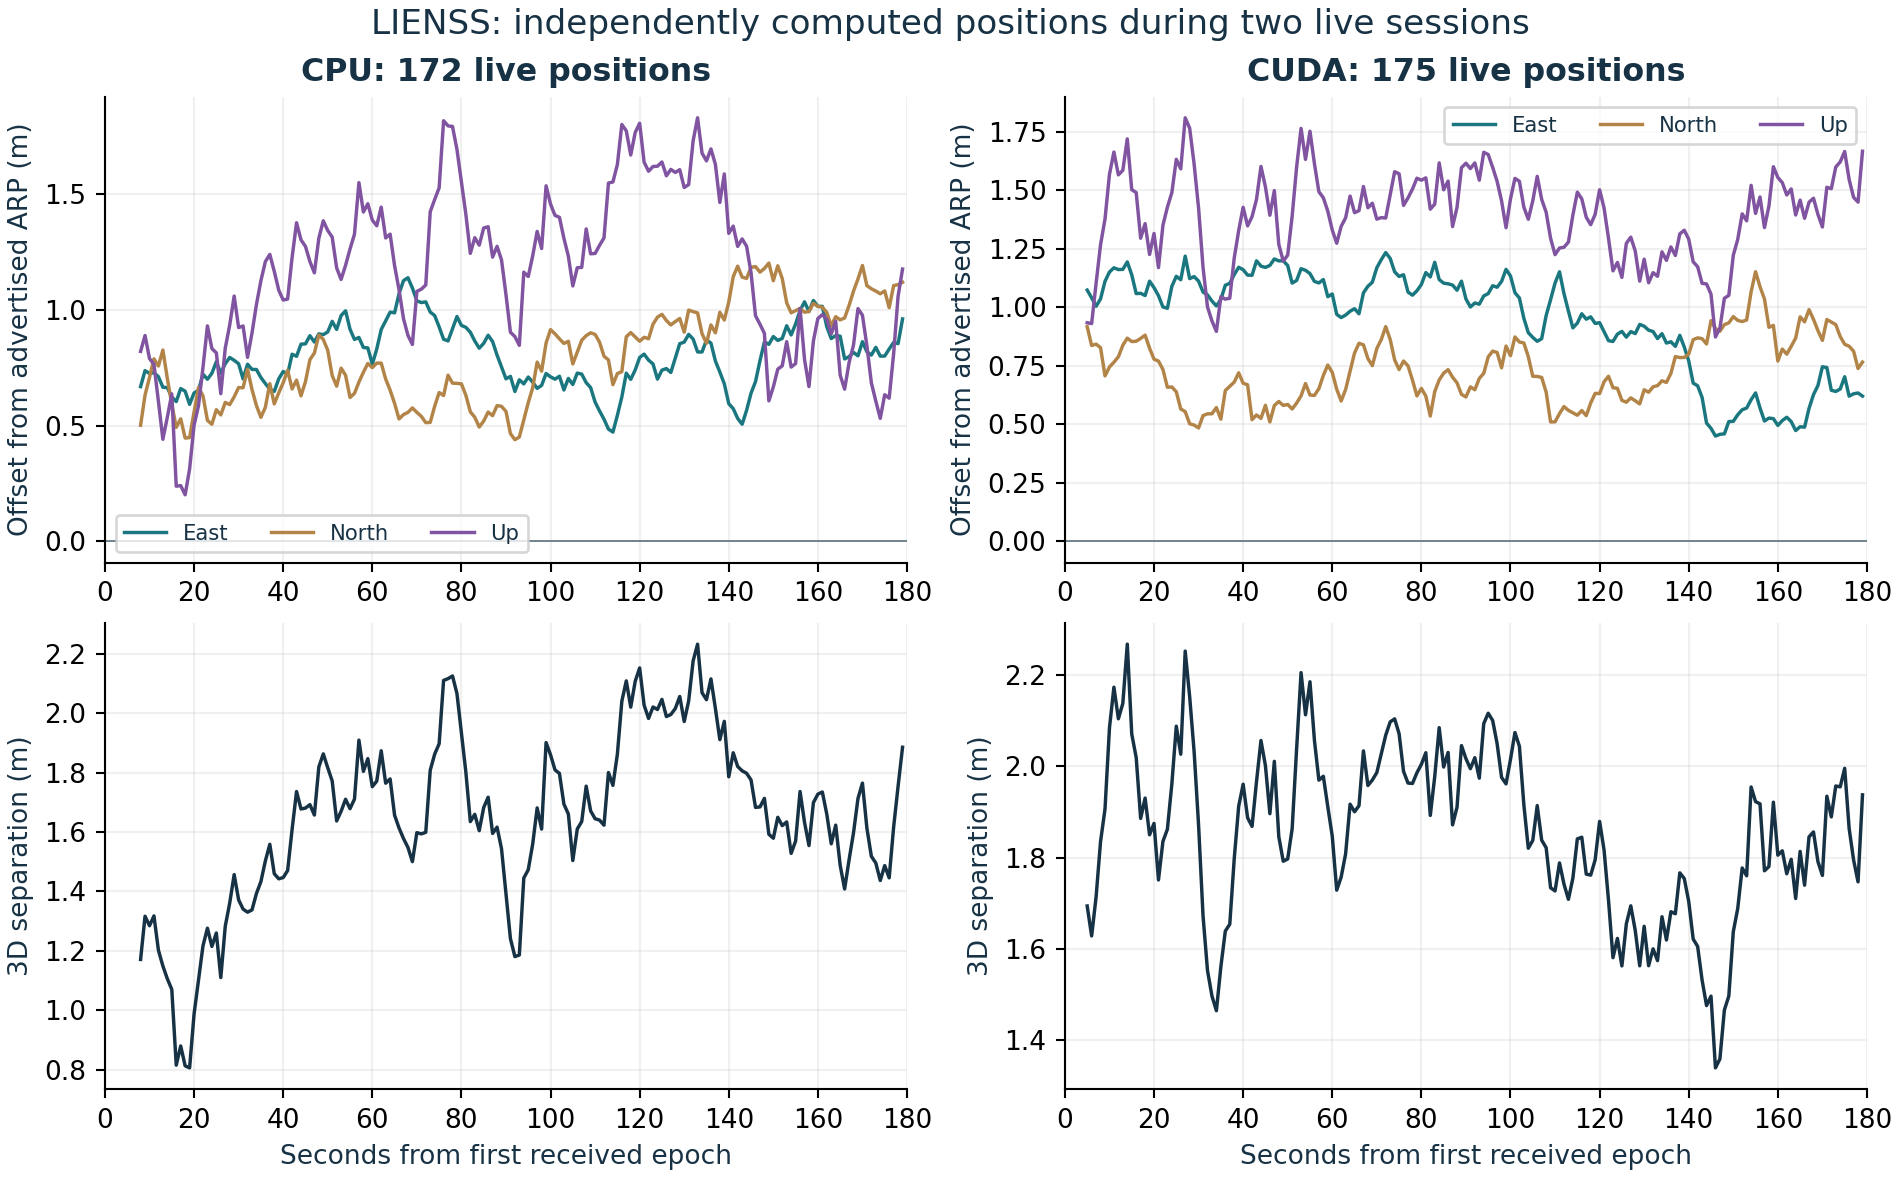
\includegraphics[width=\textwidth]{figures/live_position_evidence.png}
\end{center}
\textbf{Figure.} East/North/Up and three-dimensional separation from the advertised
ARP in the two actual live sessions. The blank beginning is ephemeris warmup;
no position is fabricated for it. These are different time windows, so their
physical differences are not a CPU-versus-GPU numerical comparison.

For that numerical comparison, the same final raw capture was replayed through
both backends with the same preparation model and receive order. Both produced
175 positions from 180 epochs; their maximum ECEF/clock component difference was
$1.21\times10^{-8}$ m. Live CUDA and its archived-byte replay also passed the same
epoch/status/position comparison. \path{results/live_cross_backend.json} records it.

The independent published RTKLIB \code{convbin} decoded each capture to RINEX.
The final CPU and CUDA decoded satellite/epoch sets matched exactly; 1980 and
2094 common C1C ranges agreed to 0.279 mm, within RINEX decimal rounding. Respectively
280 and 588 ephemeris numeric fields agreed. A separate pyrtcm field audit on the
five-minute source capture passed 96,880 comparisons. The orbit/clock oracle
matched eight satellite positions to 0.578 mm and clocks to 0.000438 ns, limited
by its printed output precision. Source hashes and commands are retained.

\clearpage
\subsection{Regression, real-model checks and retained state connection}
The older GSI recording solved all 120 real epochs from ECEF zero. Its raw physical
model and weight-isolation experiment are described with the equations above.
Prepared final live CPU observations passed 3,324 independent Householder checks
across all 180 epochs, with maximum state-component difference below
$8.4\times10^{-9}$ m. All partial/warmup statuses were retained. The persistent
CUDA worker processed those same real final-pass inputs under Compute Sanitizer:
zero memory errors, 180 responses and 1,048 independent checks.

Current native builds passed all three CTest suites on CPU and CUDA. Python passed
118 test methods. The persistent-interface regression passed 6,861 comparisons
per backend, including rejected requests followed by successful recovery.
The existing texture/global CUDA paths also passed independent comparison and
Compute Sanitizer through \code{validate\_gpu.py --sanitizer}. Analytic/parser tests
cover wrong CRC, fragments, missing data, stream truncation, HTTP chunking,
reconnection, callback failure, stale epochs, native failure and cold-start rules.

Independent NumPy re-solves verified all 698 converged outer passes across both
final live sessions to $1.40\times10^{-8}$ m per component. The physical audit
checked 6,284 prepared rows, including original code, correction signs and proof
that every chosen 1019 issue had already arrived before its epoch was solved.
All 347 published fixes preserve the corrected reception-time equation.

The same live position records also cross the retained CGK-R1 handoff after
capture. Only completed positions enter that downstream replay; omitted warmup
epochs remain listed in its manifest. ENU is anchored at the first computed
position, never at the advertised ARP. Original IDs, ECEF, receiver clock and full
time remain attached. Both key layouts are emitted wherever the chart is defined.
The stationary demonstration does not require the word state to switch, and its
modeled mechanics are not interpreted as a measured receiver velocity. The final
CPU bridge retained 172 fixes and listed eight warmup omissions; its native batch
position/clock replay exactly matched the stream. CGK replay passed 16,684 field
comparisons, and a separate binding audit passed 1,042 checks. The word remained
$q=0$ in this static session. Both keys were emitted for 153 positions; 19
remained inside the chart core. These facts do not assert dynamic switching.

\textbf{Evidence index.} \path{results/validation_status.json} links current
reports and their hashes. \path{results/network_probes/} contains the independent
conversion, raw-field and RTKLIB comparisons. \path{source/live_data/README.md}
records data provenance and third-party attribution. Parent 3.6.1.7 totals in
the following chapters are explicitly historical and are not added to these
live-session results. The original sibling release remains unchanged.


\clearpage
\subsection{Scope of the resulting navigation kernel}
This release now contains real raw-data ingestion, satellite ephemeris propagation,
explicit physical code corrections, continuous native position/clock computation,
and independent real-observation evidence. It is a working single-point GPS L1
receiver backend. The validation uses a static public base station and an older
real receiver recording; it does not establish moving-receiver field performance.

The retained CGK-R1 equations provide an explicit geometry/word/mechanics model
downstream. Their modeled motion must remain distinguishable from receiver
measurements; ASA/NA and JK feedback alone do not add independent observables or
cancel unknown GNSS errors. Full ECEF, Up, receiver clock, linear time and both
UGTS key layouts remain represented under their existing contracts.

Additional applications can consume the position/time records: maps, logging,
spatial queries, digital twins or a later motion estimator. A moving local satnav
still needs its own receiver observation source; higher precision needs additional
models such as differential corrections or carrier ambiguities. RTK/PPP, Doppler
velocity, multi-constellation clock states, map routing and calibrated antenna/code
bias estimation are separate implementations. The delivered static-session
statistics and formal covariance do not stand in for those missing capabilities.

\begin{center}
\begin{tabularx}{\textwidth}{@{}P{.28\textwidth}YY@{}}\toprule
\textbf{Use case} & \textbf{Available output or mechanism} & \textbf{Additional work for deployment}\\\midrule
Remote position logging & Live ECEF, clock, full time, raw observations and reproducible lineage. & Long-duration operation, service monitoring and application storage.\\
Local moving satnav & Executable receiver-to-position backend. & Local receiver observations, motion validation and the desired map/routing interface.\\
Spatial indexing & ENU/Up, chart state, full time and both exact UGTS key layouts. & Application database, spatial extent and query policy.\\
Digital simulation & Editable literal equations and coupled geometry/mechanics. & Calibrated model parameters and validation against the intended system.\\
Precise positioning & Raw code and available carrier metadata retained. & Differential/precise corrections, bias models and ambiguity estimation.\\\bottomrule
\end{tabularx}
\end{center}
\clearpage
